\chapter{Esperimenti di simulazione}\label{chp:esperimenti-simulazione}
In accordo agli obiettivi dello studio, per la progettazione degli esperimenti di simulazione, è stata considerata unicamente l'analisi dello stato transiente del sistema. Infatti, perderebbe di significato considerare lo stato stazionario per determinare il numero minimo di serventi necessari affinché vengano soddisfatti i QoS descritti nel capitolo \ref{chp:obiettivi}. Questo perché in una giornata lavorativa, assunta pari ad otto ore, il sistema non riesce a raggiungere lo stato stazionario prima che si verifichi la condizione di scarico (\textit{"close the door"}) ed inoltre rimane forte l'influenza delle condizioni iniziali. 

Per completezza, nella sezione \ref{sec:esperimenti-simulazione-stazionario} è mostrato il raggiungimento della stazionarietà da parte del sistema. 

\section{Progetto degli esperimenti}\label{sec:esperimenti-simulazione-1}
Per realizzare l'analisi transiente del sistema è stata adottata la tecnica \textit{replication}, utilizzando i seguenti parametri:
\begin{itemize}
\item \texttt{TERM\_INIT\_SEED = 9}, settato unicamente a inizio simulazione al fine di rendere le repliche indipendenti tra loro.
\item \texttt{ENSEMBLE\_SIZE = 300}, al fine di perdere la dipendenza dal seme iniziale pur mantenendo la variabilità naturale del fenomeno osservato.
\item \texttt{START = 0} e \texttt{STOP = 480} come descritto in sezione \ref{sec:modello-computazionale-clock}.
\end{itemize}

Inoltre:
\begin{itemize}
\item È stato utilizzato il programma \texttt{estimate} per il calcolo delle realizzazioni degli intervalli di confidenza.
\item È stato utilizzato il programma \texttt{uvs} per il calcolo di media e deviazione standard.
\end{itemize}

Di seguito sono riportate le descrizioni degli esperimenti di simulazione compiuti.

\subsection*{Numero minimo di sportelli}
Per individuare il numero minimo $M^*$ di sportelli da mantenere operativi in una giornata lavorativa, al fine di soddisfare i QoS (cap. \ref{chp:obiettivi}), un primo esperimento condotto è stato quello di analizzare l'attesa media di ciascun flusso d'arrivo al variare di $M$.

A tal proposito, è stato simulato il sistema per un'intera giornata di lavoro, assumendo che i clienti iniziassero ad arrivare all'ufficio postale \textbf{solo} successivamente all'apertura (sistema inizialmente scarico).

\subsection*{Attesa nell'arco della giornata a partire dal sistema scarico}
Una volta individuato il valore $M^*$, è stata studiata l'evoluzione dell'attesa media per ciascun flusso d'arrivo all'avanzare del tempo di simulazione.

Per realizzare quest'esperimento, la simulazione è stata arrestata ogni:
\begin{equation}
\begin{array}{l l l l l l}
45\ min, & 45 + 2\ min, & 45 + 2^2\ min, & \dots, & 45 + 2^8\ min, & 480\ min
\end{array}
\end{equation}
per le seguenti motivazioni:
\begin{itemize}
\item È stato scelto di partire da $45\ min$ per consentire la formazione delle code (poiché il sistema parte da scarico).
\item La crescita esponenziale per potenze di 2 successive permette di avere una visione a grana fine negli intervalli iniziali dove, essendo il sistema in fase di caricamento, è più probabile vi sia una maggiore variabilità dell'andamento del tempo di coda. 
\end{itemize}

\subsection*{Attesa nell'arco della giornata a partire da condizioni iniziali non nulle}
Per enfatizzare l'impatto delle condizioni iniziali sulle prestazioni del sistema, è stato replicato l'esperimento precedente assumendo che all'apertura dell'ufficio postale vi fossero già dei clienti in attesa di essere serviti.

Per ciascuna tipologia di flusso, il numero iniziale di clienti è stato impostato pari alla parte intera superiore della rispettiva popolazione media calcolata a partire da condizioni iniziali nulle, ovvero:
\begin{equation}
Customers_i(0) = \lceil\ \bar{l}_i\ \rceil
\end{equation}
in riferimento alla definizione nella \ref{eqn:modello-specifiche-2}.

Da cui:
\begin{equation}
\begin{array}{l l l}
Customers_0(0) = 1, & Customers_1(0) = 1, & Customers_2(0) = 2, \\
Customers_3(0) = 3, & Customers_4(0) = 1, & Customers_5(0) = 2
\end{array}
\end{equation}
	
\section{Esecuzione degli esperimenti ed analisi degli output}
\subsection*{Numero minimo di sportelli}
I risultati dell'esperimento condotto sono riportati sia in forma tabellare (tab. \ref{table:esperimenti-simulazione-1}) che in forma grafica (fig. \ref{fig:esperimenti-simulazione-1}).

È immediato osservare che per rispettare i requisiti di qualità stabiliti nel capitolo \ref{chp:obiettivi}, mostrati nei grafici tramite linee rosse tratteggiate, il numero minimo di serventi è $M^* = 4$. Infatti, dalla figura \ref{fig:esperimenti-simulazione-1d} si evince che con $M = 3$ non è possibile rispettare il QoS (in tabella \ref{table:esperimenti-simulazione-1a} è evidenziato in {\color{red}rosso} il valore di  attesa che lo supera).

È opportuno notare che le ampiezze delle realizzazioni degli intervalli di confidenza nel caso di \sr{} sono maggiori rispetto ai casi di \uo{} e \pp{}. Ciò è dovuto all'inferiore frequenza di arrivo e quindi alla ridotta quantità di dati utilizzati per il calcolo delle stime.

\subsection*{Attesa nell'arco della giornata a partire dal sistema scarico}
I risultati dell'esperimento condotto sono riportati sia in forma tabellare (tab. \ref{table:esperimenti-simulazione-2}) che in forma grafica (fig. \ref{fig:esperimenti-simulazione-2}).

Per la realizzazione dei grafici è stato attivato il meccanismo di svuotamento del sistema esclusivamente nell'ultima run perché, solo al superamento del tempo di simulazione $\tau$, si verifica la condizione di blocco degli arrivi (\textit{"close the door"}) e quindi il sistema deve essere riportato alle condizioni iniziali. Questo perché, nel momento in cui viene arrestata la simulazione ad un istante $t$, si è interessati ai soli eventi che occorrono in $(0, t]$ e non a quelli appartenenti a $(t, t + \Delta]$ che rappresenta l'intervallo di tempo necessario a svuotare il sistema.

Di seguito è riportata una serie di osservazioni relative ai risultati ottenuti:
\begin{itemize}
\item Il fatto che le curve, in corrispondenza $t = \tau = 480\ min$, intersechino i rispettivi valori medi (mostrati tramite linee rosse tratteggiate) rappresenta un consistency check per il simulatore, perché tali sono stati computati su finestre di medesima ampiezza.
\item Per quanto riguarda i ticket \uo{} e \pp{}, esiste una correlazione tra la pendenza delle curve e la priorità del flusso corrispondente. La spiegazione di questo fenomeno è data dal fatto che flussi prioritari impiegano meno tempo a stabilizzarsi poiché rallentati da un numero inferiore di richieste.

Ad esempio, in figura \ref{fig:esperimenti-simulazione-2a} il valore medio giornaliero ricade nell'intervallo della misura effettuata a circa tre ore dall'apertura, mentre lo stesso si verifica in figura \ref{fig:esperimenti-simulazione-2d} dopo circa cinque.
\item Poiché l'utilizzazione dei ticket \sr{} è bassa, mentre quella di \uo{} e \pp{} è alta, è molto probabile che inizialmente all'arrivo di un ticket del primo tipo, il server dedicato stia processando una richiesta degli altri due. Questo fenomeno è enfatizzato dal fatto che inizialmente non vi sono clienti nel sistema.

Con l'avanzare del tempo, invece, è sempre meno probabile che ticket di tipo \uo{} oppure \pp{} rallentino quelli di \sr{}, per via dello stabilizzarsi dell'occupazione. 
\end{itemize}

\subsection*{Attesa nell'arco della giornata a partire da condizioni iniziali non nulle}
I risultati dell'esperimento condotto sono riportati sia in forma tabellare (tab. \ref{table:esperimenti-simulazione-3}) che in forma grafica (fig. \ref{fig:esperimenti-simulazione-3}).

Di seguito è riportata una serie di osservazioni relative ai risultati ottenuti:
\begin{itemize}
\item Rispetto all'esperimento precedente, le curve relative a ticket \uo{} \textsl{BancoPosta} e \pp{} \textsl{BancoPosta} mostrano una traslazione che anticipa l'istante di tempo in cui il valore medio ricade per la prima volta all'interno di un intervallo di confidenza stimato.

Poiché le code considerate hanno la priorità maggiore, l'andamento delle corrispondenti curve non risente della presenza di condizioni iniziali non nulle, perché le richieste ad esse appartenenti non subiscono ritardi dovuti alla presenza di altre di diverso tipo.
\item Le restanti quattro curve mostrano un andamento molto simile fra loro, caratterizzato da un primo periodo di crescita seguito da un successivo di decrescita verso il valore stazionario. Tale, però, potrebbe essere osservato soltanto simulando per un intervallo temporale più ampio.

Presumibilmente, il picco presente in ogni grafico è associato all'istante temporale in cui l'impatto delle condizioni iniziali sulle prestazioni del sistema comincia ad affievolirsi. Il fatto che l'istante d'occorrenza del picco è inversamente proporzionale alla priorità del flusso avvalora ulteriormente questa congettura, infatti:
\begin{itemize}
\item Il picco dell'attesa sperimentato da \uo{} standard si verifica in anticipo rispetto a quello di \pp{} standard.
\item Il picco dell'attesa sperimentato da \sr{} \textsl{BancoPosta} si verifica in anticipo rispetto a quello di \sr{} standard.
\end{itemize}
\end{itemize}

\section{Raggiungimento dello stato stazionario}\label{sec:esperimenti-simulazione-stazionario}
Per mostrare il raggiungimento dello stato stazionario da parte del sistema è stata adottata la tecnica \textit{batch means}, utilizzando i seguenti parametri:
\begin{itemize}
\item \texttt{STAT\_INIT\_SEED = 12345}.
\item \texttt{B = 960}, è stato notato essere il giusto compromesso fra il mantenimento della variabilità naturale del fenomeno osservato e l'indipendenza tra batch successivi.
\item \texttt{K = 64}, come da linee guida, al fine di rendere le statistiche campionate indipendenti dalle condizioni iniziali ed ottenere intervalli di confidenza significativi.
\item \texttt{START = 0} e $\mathtt{STOP = B \cdot K = 61440}$.
\end{itemize}

Inoltre, è stato utilizzato il programma \texttt{estimate} per il calcolo delle realizzazioni degli intervalli di confidenza.

I risultati riportati sia in forma tabellare (tab. \ref{table:esperimenti-simulazione-4}) che in forma grafica (fig. \ref{fig:esperimenti-simulazione-4}) mostrano l'andamento dell'attesa media:
\begin{itemize}
\item Per ticket di tipo \uo{} e \pp{} (tab. \ref{table:esperimenti-simulazione-4a} e fig. \ref{fig:esperimenti-simulazione-4a})
\item Per ticket di tipo \sr{} (tab. \ref{table:esperimenti-simulazione-4a} e fig. \ref{fig:esperimenti-simulazione-4b})
\end{itemize}
al variare del numero di batch considerati fino a raggiungere il valore di \texttt{K} sopra definito.

I dati raccolti confermano quanto detto ad inizio capitolo, ovvero è possibile raggiungere lo stato stazionario soltanto prendendo in considerazione finestre temporali più ampie dei $480\ min$ giornalieri.

\section{Grafici e tabelle}
\begin{table}[ht]
\centering
\begin{subtable}{0.33\textwidth}
\centering
{\tablecolors
\begin{tabular}{|c|c|c|}
\hline
$i$ & Media & Dev. std. \\
\hline
0 & 6.617 & 2.665 \\
\hline
1 & 9.249 & 5.187 \\
\hline
2 & 31.741 & 23.652 \\
\hline
3 & {\color{red}150.841} & 87.434 \\
\hline
4 & 15.214 & 9.978 \\
\hline
5 & 31.319 & 21.485 \\
\hline
\end{tabular}}
\caption{$M = 3$}
\label{table:esperimenti-simulazione-1a}
\end{subtable}%
\begin{subtable}{0.33\textwidth}
\centering
{\tablecolors
\begin{tabular}{|c|c|c|}
\hline
$i$ & Media & Dev. std. \\
\hline
0 & 3.209 & 1.773 \\
\hline
1 & 3.926 & 2.861 \\
\hline
2 & 8.928 & 7.196 \\
\hline
3 & 33.333 & 35.001 \\
\hline
4 & 14.057 & 10.772 \\
\hline
5 & 29.007 & 22.434 \\
\hline
\end{tabular}}
\caption{$M = 4$}
\end{subtable}%
\begin{subtable}{0.33\textwidth}
\centering
{\tablecolors
\begin{tabular}{|c|c|c|}
\hline
$i$ & Media & Dev. std. \\
\hline
0 & 1.270 & 1.156 \\
\hline
1 & 1.566 & 1.656 \\
\hline
2 & 2.758 & 2.490 \\
\hline
3 & 6.909 & 9.763 \\
\hline
4 & 11.510 & 11.065 \\
\hline
5 & 22.638 & 19.546 \\
\hline
\end{tabular}}
\caption{$M = 5$}
\end{subtable}
\caption{Attesa espressa in minuti, per ciascun flusso $i$, al variare di $M$}
\label{table:esperimenti-simulazione-1}
\end{table}

\begin{figure}[ht]
\centering
\begin{subfigure}[b]{0.475\textwidth}
\centering
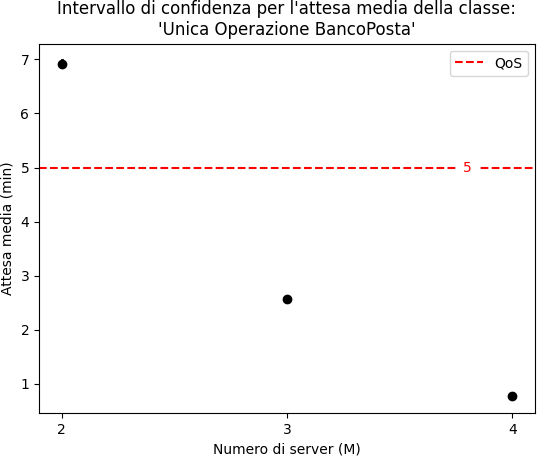
\includegraphics[width=\textwidth]{plots/d0-trans}
\caption{\uo{} BP}    
\end{subfigure}
\hfill    
\begin{subfigure}[b]{0.475\textwidth}  
\centering 
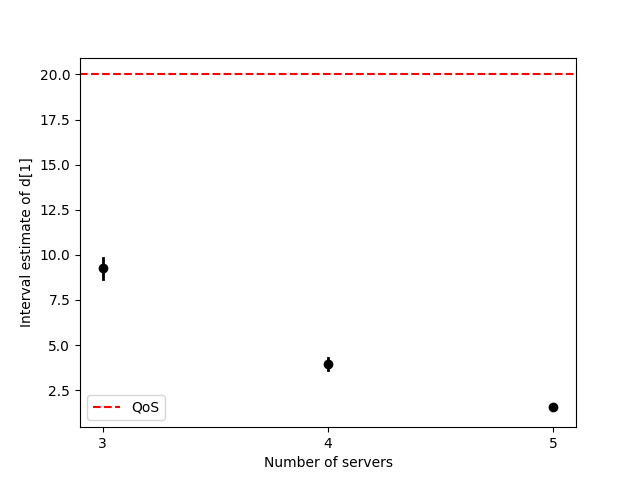
\includegraphics[width=\textwidth]{plots/d1-trans}
\caption{\pp{} BP}    
\end{subfigure}

\vskip\baselineskip

\begin{subfigure}[b]{0.475\textwidth}   
\centering 
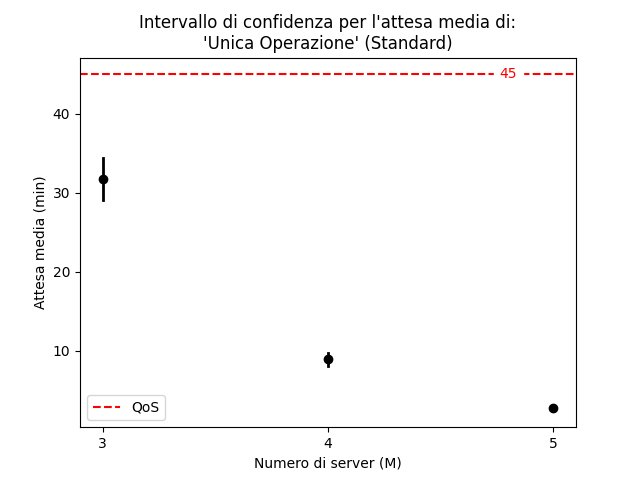
\includegraphics[width=\textwidth]{plots/d2-trans}
\caption{\uo{} STD}    
\end{subfigure}
\hfill
\begin{subfigure}[b]{0.475\textwidth}   
\centering 
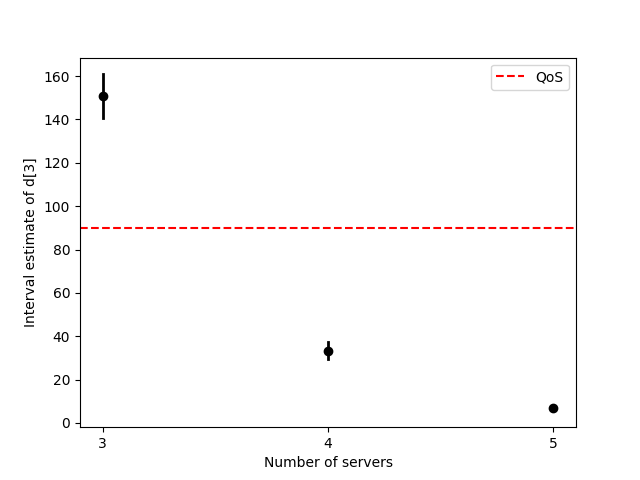
\includegraphics[width=\textwidth]{plots/d3-trans}
\caption{\pp{} STD}
\label{fig:esperimenti-simulazione-1d}  
\end{subfigure}

\vskip\baselineskip

\begin{subfigure}[b]{0.475\textwidth}   
\centering 
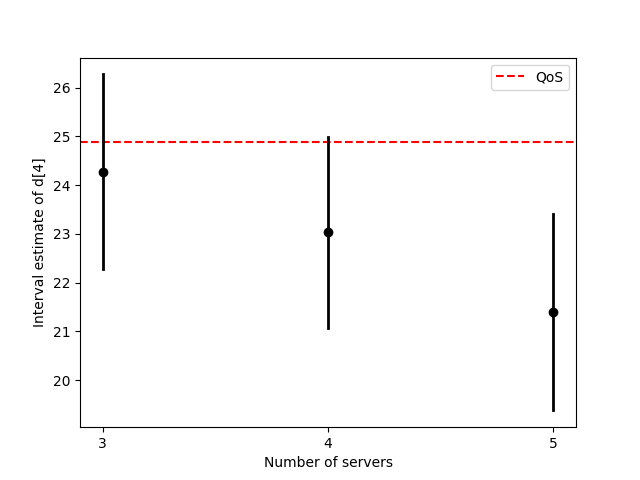
\includegraphics[width=\textwidth]{plots/d4-trans}
\caption{\sr{} BP}    
\end{subfigure}
\hfill
\begin{subfigure}[b]{0.475\textwidth}   
\centering 
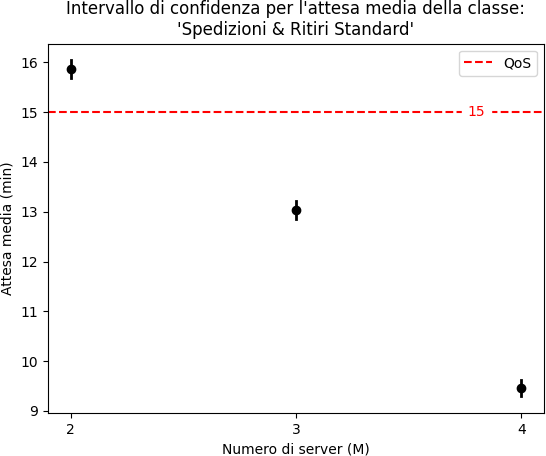
\includegraphics[width=\textwidth]{plots/d5-trans}
\caption{\sr{} STD}    
\end{subfigure}
\caption{Attesa espressa in minuti, per ciascun flusso, al variare di $M$}
\label{fig:esperimenti-simulazione-1}
\end{figure}

\begin{table}[ht]
\centering
\begin{subtable}{0.33\textwidth}
\centering
{\tablecolors
\begin{tabular}{|c|c|c|}
\hline
$t$ & Media & Dev. std. \\
\hline
45 & 0.414 & 1.548 \\
\hline
47 & 0.868 & 2.691 \\
\hline
49 & 0.471 & 1.418 \\
\hline
53 & 0.691 & 2.104 \\
\hline
61 & 1.295 & 3.495 \\
\hline
77 & 1.771 & 4.198 \\
\hline
109 & 1.858 & 2.725 \\
\hline
173 & 2.949 & 4.596 \\
\hline
301 & 3.131 & 3.077 \\
\hline
480 & 3.209 & 1.773 \\
\hline
\end{tabular}}
\caption{\uo{} BP}
\end{subtable}%
\begin{subtable}{0.33\textwidth}
\centering
{\tablecolors
\begin{tabular}{|c|c|c|}
\hline
$t$ & Media & Dev. std. \\
\hline
45 & 0.320 & 1.307 \\
\hline
47 & 0.585 & 2.495 \\
\hline
49 & 0.493 & 2.375 \\
\hline
53 & 0.614 & 2.129 \\
\hline
61 & 0.993 & 2.977 \\
\hline
77 & 1.604 & 4.195 \\
\hline
109 & 1.863 & 4.169 \\
\hline
173 & 3.502 & 5.224 \\
\hline
301 & 3.907 & 3.810 \\
\hline
480 & 3.926 & 2.861 \\
\hline
\end{tabular}}
\caption{\pp{} BP}
\end{subtable}%
\begin{subtable}{0.33\textwidth}
\centering
{\tablecolors
\begin{tabular}{|c|c|c|}
\hline
$t$ & Media & Dev. std. \\
\hline
45 & 1.968 & 6.078 \\
\hline
47 & 2.407 & 6.855 \\
\hline
49 & 2.270 & 5.500 \\
\hline
53 & 3.405 & 9.793 \\
\hline
61 & 3.400 & 7.835 \\
\hline
77 & 4.080 & 7.413 \\
\hline
109 & 5.453 & 15.151 \\
\hline
173 & 5.908 & 6.938 \\
\hline
301 & 7.457 & 7.497 \\
\hline
480 & 8.928 & 7.196 \\
\hline
\end{tabular}}
\caption{\uo{} STD}
\end{subtable}

\vskip\baselineskip

\begin{subtable}{0.33\textwidth}
\centering
{\tablecolors
\begin{tabular}{|c|c|c|}
\hline
$t$ & Media & Dev. std. \\
\hline
45 & 2.069 & 6.163 \\
\hline
47 & 3.473 & 12.020 \\
\hline
49 & 3.590 & 10.134 \\
\hline
53 & 3.493 & 8.610 \\
\hline
61 & 6.900 & 21.047 \\
\hline
77 & 9.169 & 20.923 \\
\hline
109 & 11.868 & 25.342 \\
\hline
173 & 20.825 & 46.042 \\
\hline
301 & 29.093 & 43.216 \\
\hline
480 & 33.333 & 35.001 \\
\hline
\end{tabular}}
\caption{\pp{} STD}
\end{subtable}%
\begin{subtable}{0.33\textwidth}
\centering
{\tablecolors
\begin{tabular}{|c|c|c|}
\hline
$t$ & Media & Dev. std. \\
\hline
45 & 0.688 & 3.683 \\
\hline
47 & 0.928 & 4.045 \\
\hline
49 & 0.658 & 3.006 \\
\hline
53 & 1.228 & 5.497 \\
\hline
61 & 1.791 & 6.327 \\
\hline
77 & 1.909 & 5.340 \\
\hline
109 & 4.130 & 9.135 \\
\hline
173 & 10.251 & 17.556 \\
\hline
301 & 13.781 & 15.646 \\
\hline
480 & 14.057 & 10.772 \\
\hline
\end{tabular}}
\caption{\sr{} BP}
\end{subtable}%
\begin{subtable}{0.33\textwidth}
\centering
{\tablecolors
\begin{tabular}{|c|c|c|}
\hline
$t$ & Media & Dev. std. \\
\hline
45 & 2.138 & 6.692 \\
\hline
47 & 2.680 & 8.163 \\
\hline
49 & 3.629 & 11.080 \\
\hline
53 & 5.105 & 14.060 \\
\hline
61 & 5.224 & 12.921 \\
\hline
77 & 8.465 & 15.294 \\
\hline
109 & 17.582 & 28.532 \\
\hline
173 & 28.505 & 41.330 \\
\hline
301 & 30.962 & 48.066 \\
\hline
480 & 29.007 & 22.434 \\
\hline
\end{tabular}}
\caption{\sr{} STD}
\end{subtable}
\caption{Attesa in minuti in funzione di $t$ (sistema inizialmente scarico)}
\label{table:esperimenti-simulazione-2}
\end{table}

\begin{figure}[ht]
\centering
\begin{subfigure}[b]{0.475\textwidth}
\centering
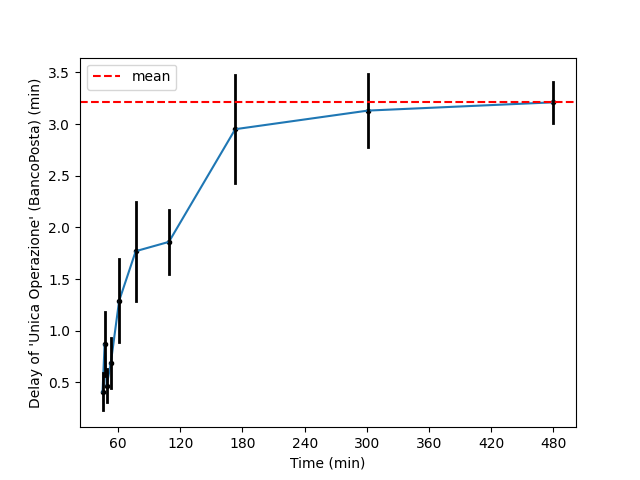
\includegraphics[width=\textwidth]{plots/day-from-empty-0}
\caption{\uo{} BP}    
\label{fig:esperimenti-simulazione-2a}
\end{subfigure}
\hfill    
\begin{subfigure}[b]{0.475\textwidth}  
\centering 
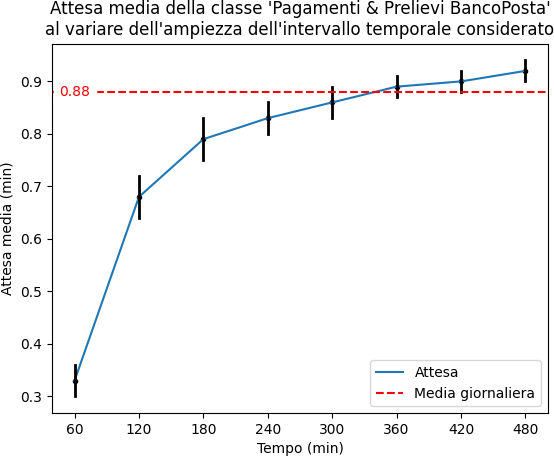
\includegraphics[width=\textwidth]{plots/day-from-empty-1}
\caption{\pp{} BP}    
\end{subfigure}

\vskip\baselineskip

\begin{subfigure}[b]{0.475\textwidth}   
\centering 
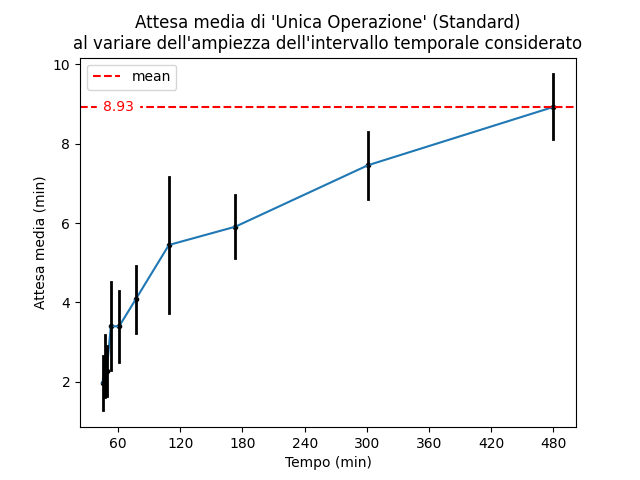
\includegraphics[width=\textwidth]{plots/day-from-empty-2}
\caption{\uo{} STD}    
\end{subfigure}
\hfill
\begin{subfigure}[b]{0.475\textwidth}   
\centering 
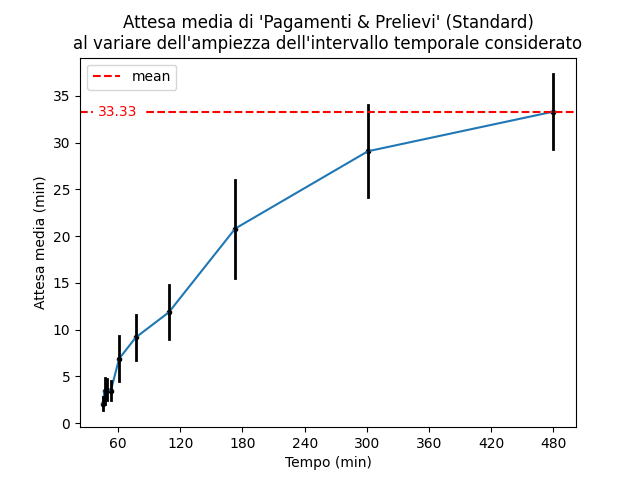
\includegraphics[width=\textwidth]{plots/day-from-empty-3}
\caption{\pp{} STD}    
\label{fig:esperimenti-simulazione-2d}
\end{subfigure}

\vskip\baselineskip

\begin{subfigure}[b]{0.475\textwidth}   
\centering 
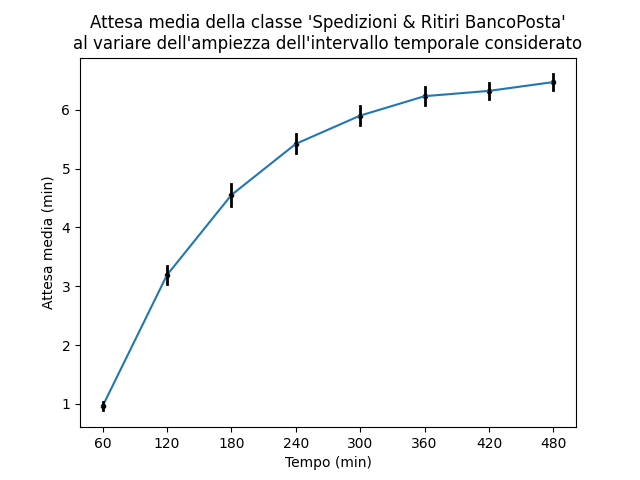
\includegraphics[width=\textwidth]{plots/day-from-empty-4}
\caption{\sr{} BP}    
\end{subfigure}
\hfill
\begin{subfigure}[b]{0.475\textwidth}   
\centering 
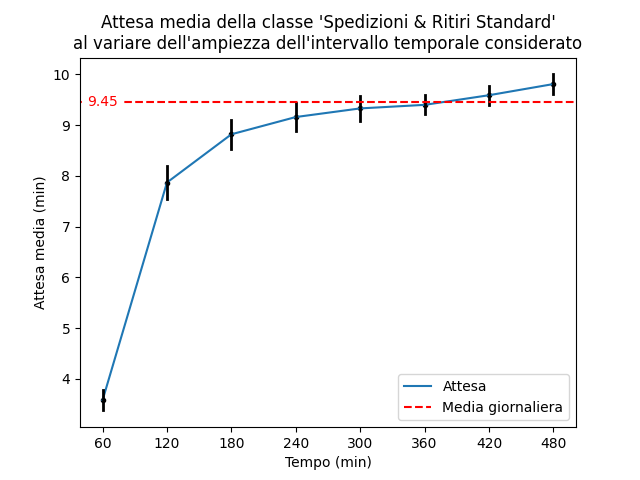
\includegraphics[width=\textwidth]{plots/day-from-empty-5}
\caption{\sr{} STD}    
\end{subfigure}
\caption{Attesa in minuti in funzione di $t$ (sistema inizialmente scarico)}
\label{fig:esperimenti-simulazione-2}
\end{figure}

\begin{table}[ht]
\centering
\begin{subtable}{0.33\textwidth}
\centering
{\tablecolors
\begin{tabular}{|c|c|c|}
\hline
$t$ & Media & Dev. std. \\
\hline
45 & 2.095 & 3.091 \\
\hline
47 & 1.979 & 2.889 \\
\hline
49 & 2.130 & 3.176 \\
\hline
53 & 2.211 & 2.842 \\
\hline
61 & 2.474 & 2.794 \\
\hline
77 & 3.084 & 8.423 \\
\hline
109 & 3.331 & 3.045 \\
\hline
173 & 3.527 & 2.302 \\
\hline
301 & 3.910 & 2.179 \\
\hline
480 & 4.128 & 1.871 \\
\hline
\end{tabular}}
\caption{\uo{} BP}
\end{subtable}%
\begin{subtable}{0.33\textwidth}
\centering
{\tablecolors
\begin{tabular}{|c|c|c|}
\hline
$t$ & Media & Dev. std. \\
\hline
45 & 2.216 & 4.123 \\
\hline
47 & 2.326 & 4.959 \\
\hline
49 & 2.534 & 5.311 \\
\hline
53 & 2.114 & 4.168 \\
\hline
61 & 2.517 & 3.389 \\
\hline
77 & 2.725 & 3.222 \\
\hline
109 & 3.671 & 4.231 \\
\hline
173 & 3.954 & 3.263 \\
\hline
301 & 4.909 & 4.298 \\
\hline
480 & 4.810 & 2.636 \\
\hline
\end{tabular}}
\caption{\pp{} BP}
\end{subtable}%
\begin{subtable}{0.33\textwidth}
\centering
{\tablecolors
\begin{tabular}{|c|c|c|}
\hline
$t$ & Media & Dev. std. \\
\hline
45 & 25.133 & 35.355 \\
\hline
47 & 27.465 & 42.575 \\
\hline
49 & 25.416 & 38.328 \\
\hline
53 & 24.629 & 36.087 \\
\hline
61 & 26.715 & 42.081 \\
\hline
77 & 20.518 & 22.150 \\
\hline
109 & 18.805 & 19.564 \\
\hline
173 & 15.111 & 9.707 \\
\hline
301 & 15.047 & 11.252 \\
\hline
480 & 13.620 & 8.898 \\
\hline
\end{tabular}}
\caption{\uo{} STD}
\end{subtable}

\vskip\baselineskip

\begin{subtable}{0.33\textwidth}
\centering
{\tablecolors
\begin{tabular}{|c|c|c|}
\hline
$t$ & Media & Dev. std. \\
\hline
45 & 52.743 & 74.041 \\
\hline
47 & 52.460 & 78.194 \\
\hline
49 & 55.243 & 77.938 \\
\hline
53 & 69.035 & 89.336 \\
\hline
61 & 85.170 & 111.186 \\
\hline
77 & 116.143 & 158.133 \\
\hline
109 & 142.648 & 180.197 \\
\hline
173 & 155.809 & 263.976 \\
\hline
301 & 117.047 & 127.858 \\
\hline
480 & 77.668 & 57.835 \\
\hline
\end{tabular}}
\caption{\pp{} STD}
\end{subtable}%
\begin{subtable}{0.33\textwidth}
\centering
{\tablecolors
\begin{tabular}{|c|c|c|}
\hline
$t$ & Media & Dev. std. \\
\hline
45 & 23.042 & 25.085 \\
\hline
47 & 20.614 & 23.718 \\
\hline
49 & 23.881 & 26.667 \\
\hline
53 & 27.914 & 31.099 \\
\hline
61 & 28.531 & 35.438 \\
\hline
77 & 30.556 & 33.375 \\
\hline
109 & 28.422 & 28.093 \\
\hline
173 & 26.623 & 21.037 \\
\hline
301 & 23.454 & 15.677 \\
\hline
480 & 21.362 & 12.061 \\
\hline
\end{tabular}}
\caption{\sr{} BP}
\end{subtable}%
\begin{subtable}{0.33\textwidth}
\centering
{\tablecolors
\begin{tabular}{|c|c|c|}
\hline
$t$ & Media & Dev. std. \\
\hline
45 & 19.805 & 44.107 \\
\hline
47 & 30.889 & 54.541 \\
\hline
49 & 23.537 & 47.689 \\
\hline
53 & 36.596 & 63.849 \\
\hline
61 & 45.917 & 73.575 \\
\hline
77 & 85.982 & 104.271 \\
\hline
109 & 120.387 & 135.340 \\
\hline
173 & 106.082 & 116.812 \\
\hline
301 & 78.264 & 98.993 \\
\hline
480 & 52.513 & 28.532 \\
\hline
\end{tabular}}
\caption{\sr{} STD}
\end{subtable}
\caption{Attesa in minuti in funzione di $t$ (sistema inizialmente \textbf{non} scarico)}
\label{table:esperimenti-simulazione-3}
\end{table}

\begin{figure}[ht]
\centering
\begin{subfigure}[b]{0.475\textwidth}
\centering
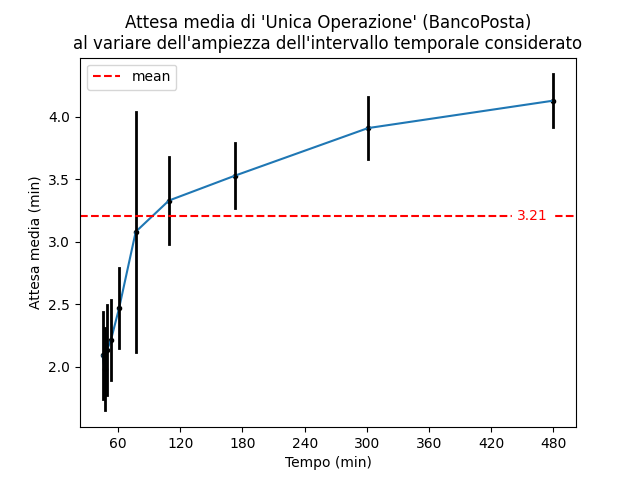
\includegraphics[width=\textwidth]{plots/day-from-mean-values-0}
\caption{\uo{} BP}
\end{subfigure}
\hfill    
\begin{subfigure}[b]{0.475\textwidth}  
\centering 
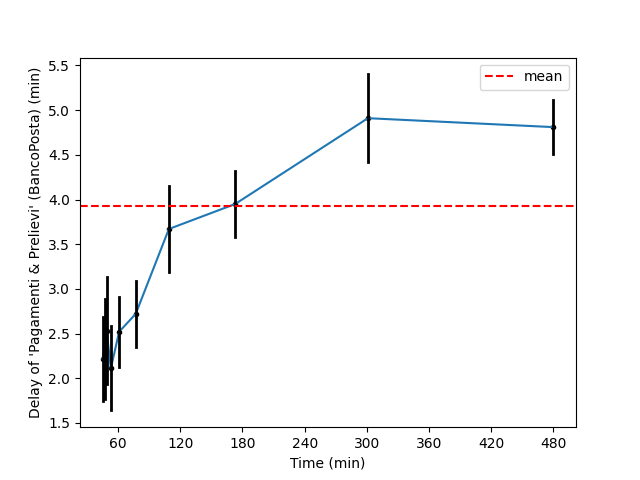
\includegraphics[width=\textwidth]{plots/day-from-mean-values-1}
\caption{\pp{} BP}
\end{subfigure}

\vskip\baselineskip

\begin{subfigure}[b]{0.475\textwidth}   
\centering 
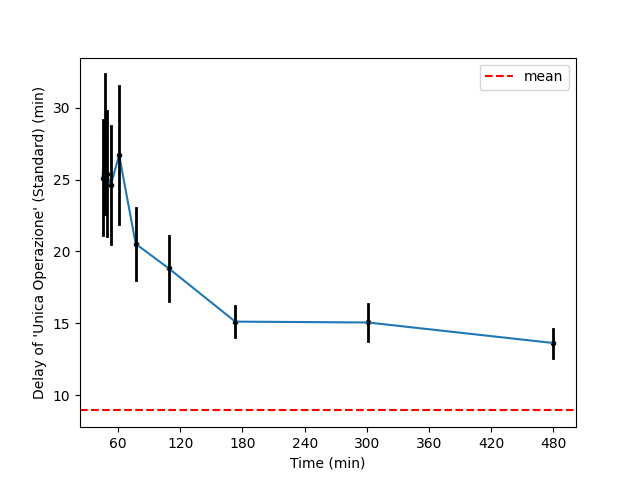
\includegraphics[width=\textwidth]{plots/day-from-mean-values-2}
\caption{\uo{} STD}
\end{subfigure}
\hfill
\begin{subfigure}[b]{0.475\textwidth}   
\centering 
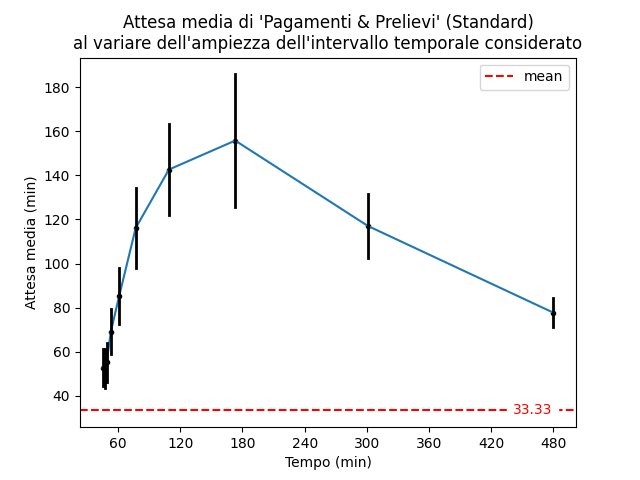
\includegraphics[width=\textwidth]{plots/day-from-mean-values-3}
\caption{\pp{} STD}
\end{subfigure}

\vskip\baselineskip

\begin{subfigure}[b]{0.475\textwidth}   
\centering 
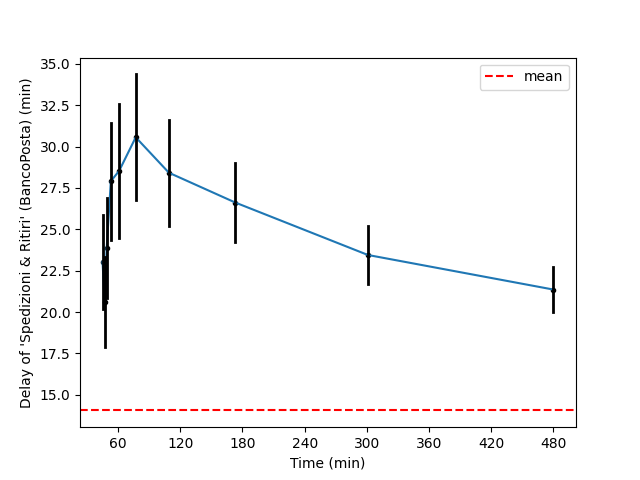
\includegraphics[width=\textwidth]{plots/day-from-mean-values-4}
\caption{\sr{} BP}
\end{subfigure}
\hfill
\begin{subfigure}[b]{0.475\textwidth}   
\centering 
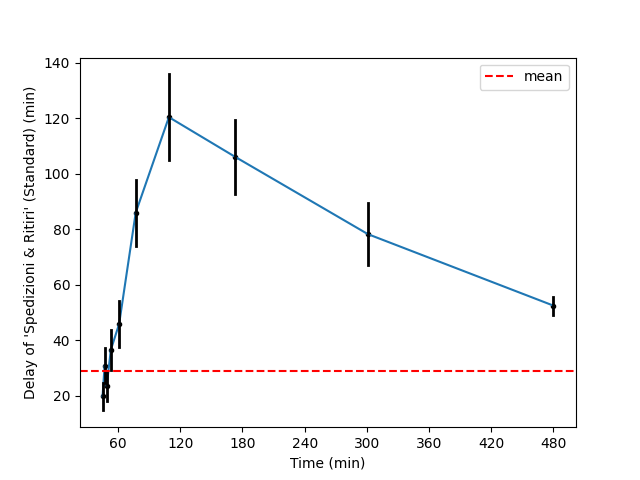
\includegraphics[width=\textwidth]{plots/day-from-mean-values-5}
\caption{\sr{} STD}
\end{subfigure}
\caption{Attesa in minuti in funzione di $t$ (sistema inizialmente \textbf{non} scarico)}
\label{fig:esperimenti-simulazione-3}
\end{figure}

\begin{table}[ht]
\centering
\begin{subtable}{0.475\textwidth}
\centering
{\tablecolors
\begin{tabular}{|c|c|c|}
\hline
$K$ & Media & Dev. std. \\
\hline
1 & 20.258 & - \\
\hline
2 & 16.041 & 4.217 \\
\hline
4 & 17.105 & 3.303 \\
\hline
8 & 40.237 & 37.398 \\
\hline
16 & 37.644 & 28.445 \\
\hline
32 & 35.328 & 34.331 \\
\hline
64 & 29.543 & 27.305 \\	
\hline
\end{tabular}}
\caption{\uo{} e \pp{}}
\label{table:esperimenti-simulazione-4a}
\end{subtable}%
\begin{subtable}{0.475\textwidth}
\centering
{\tablecolors
\begin{tabular}{|c|c|c|}
\hline
$K$ & Media & Dev. std. \\
\hline
1 & 29.430 & - \\
\hline
2 & 25.126 & 4.304 \\
\hline
4 & 27.608 & 4.663 \\
\hline
8 & 27.065 & 9.396 \\
\hline
16 & 30.917 & 14.156 \\
\hline
32 & 30.592 & 24.059 \\
\hline
64 & 30.642 & 18.991 \\
\hline
\end{tabular}}
\caption{\sr{}}
\label{table:esperimenti-simulazione-4b}
\end{subtable}
\caption{Raggiungimento dello stato stazionario del sistema}
\label{table:esperimenti-simulazione-4}
\end{table}

\begin{figure}[ht]
\centering
\begin{subfigure}[b]{0.8\textwidth}
\centering
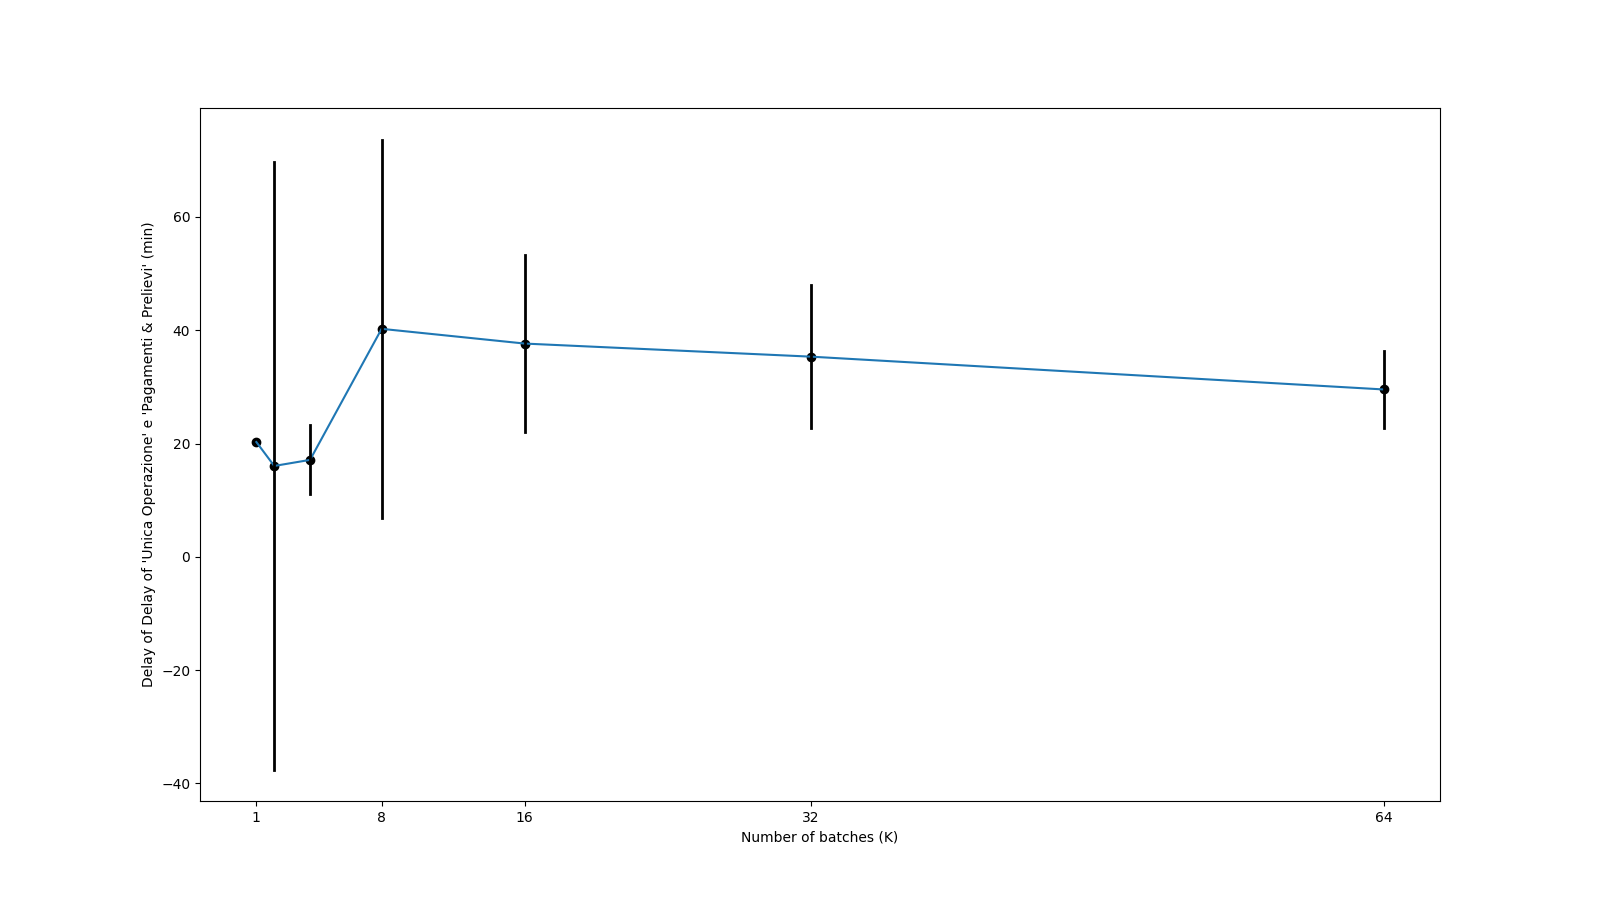
\includegraphics[width=\textwidth]{plots/d-staz-G-ic}
\caption{\uo{} e \pp{}}
\label{fig:esperimenti-simulazione-4a}
\end{subfigure}
\vskip\baselineskip    
\begin{subfigure}[b]{0.8\textwidth}  
\centering 
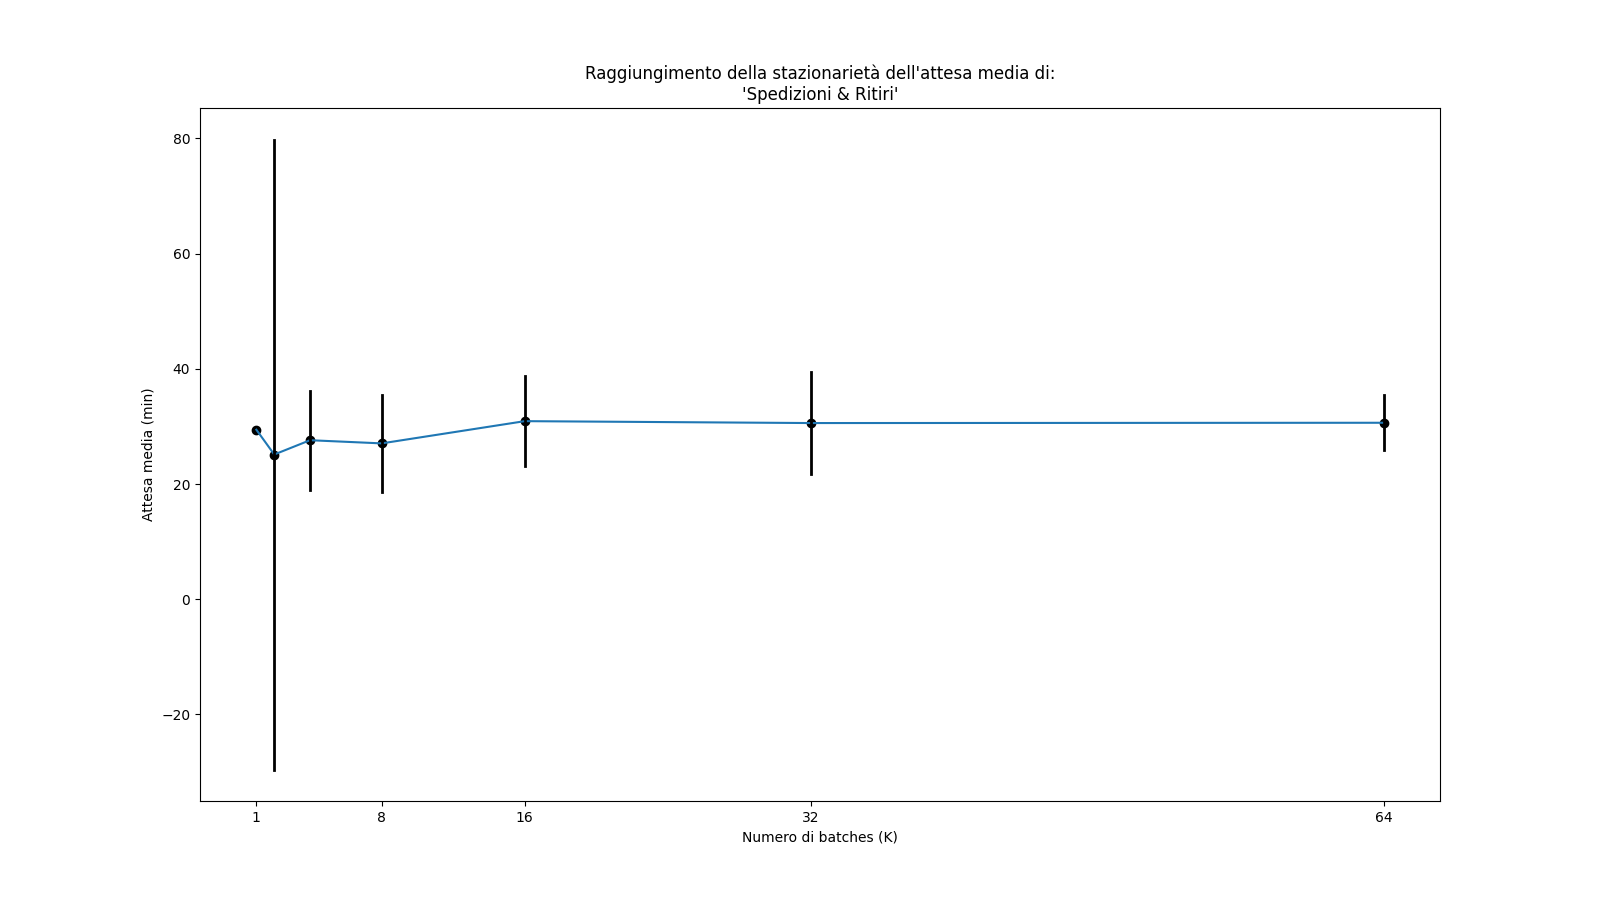
\includegraphics[width=\textwidth]{plots/d-staz-D-ic}
\caption{\sr{}}
\label{fig:esperimenti-simulazione-4b}
\end{subfigure}
\caption{Raggiungimento dello stato stazionario del sistema}
\label{fig:esperimenti-simulazione-4}
\end{figure}
